\documentclass[12pt]{article}
\usepackage[utf8]{inputenc}
\usepackage[T2A]{fontenc}
\usepackage[mongolian]{babel}
\usepackage{graphicx}

\title{Системээс хариу и-мэйл илгээх}

\begin{document}
	\section{Функциональ шаардлага}
	
	\begin{enumerate}
		\item[1] Хэрэглэгчийн функциональ шаардлага:
		\begin{itemize}
			\item И-мэйлтэй байх 
			\item Пасс сэргээх, шинээр бүртгүүлэх
			\item Мэйлээр нэвтэрч орох
			\item Нууц үг болон мэдэгдэл харах
			\item Холбоос линк дарах
			\item Он сар харагддаг байх
		\end{itemize}
	\end{enumerate}
	\begin{enumerate}
		\item[2] Системийн функциональ шаардлага:
		\begin{itemize}
			\item Мэйл илгээх загвар сонгох 
			\item Шинэчлэгдсэн пасс, линк бичих
			\item Спам мессежруу оруулахгүй байх
			\item он сар харагддаг байх
		\end{itemize}
	\end{enumerate}
	\section{Функциональ бус шаардлага}
	\begin{itemize}
		\item Өгөгдлийн сан ачааллах хугацаа нь хурдан шуурхай байх. Бүх өгөгдлүүд өгөгдлийн санд хадгалагдсан байх
		\item Вебд 1000-с 10000-хүн нэгэн зэрэг хандаж үйл ажиллагаа явуулах учир серверийн хүчин чадал өндөр байх
		\item Responsive байх
		\item хаанаас ч, хэзээ ч хандах боломжтой байх
	\end{itemize}
\begin{figure}[ht]
	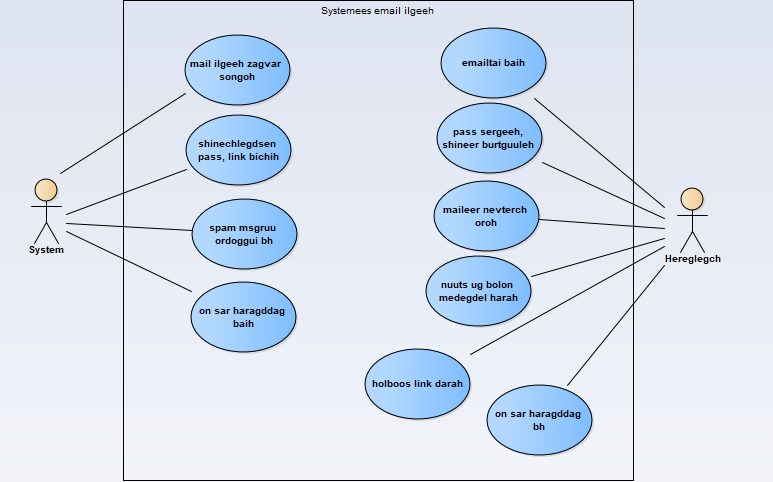
\includegraphics[width=1\linewidth]{images/email_usecase}
	\caption[Юзкейз]{Системээс хариу илгээх юзкейз}
	\label{fig:emailusecase}
\end{figure}

\end{document}
